%%%%%%%%%%%%%%%%%%%%%%%%%%%%%%%%%%%%%%%%%%%%%%%%%%%%%%%
%                  File: gdsfactory.tex               %
%                  Date: January 2026                 %
%                                                     %
%     For preparing LaTeX manuscripts for submission  %
%     to CLEO 2026 (Optica meetings and conferences)  %
%                                                     %
%%%%%%%%%%%%%%%%%%%%%%%%%%%%%%%%%%%%%%%%%%%%%%%%%%%%%%%

\documentclass[letterpaper,10pt]{article}
%% if A4 paper needed, change letterpaper to A4

\usepackage{opticameet3} %% use version 3 for proper copyright statement

%% provide authormark
\newcommand\authormark[1]{\textsuperscript{#1}}

%% standard packages and arguments should be modified as needed
\usepackage{amsmath,amssymb}
\usepackage[colorlinks=true,bookmarks=false,citecolor=blue,urlcolor=blue]{hyperref}

% ADD THE FOLLOWING COUPLE LINES INTO YOUR PREAMBLE
\let\OLDthebibliography\thebibliography%
\renewcommand\thebibliography[1]{
  \OLDthebibliography{#1}
  \setlength{\parskip}{0pt}
  \setlength{\itemsep}{0pt plus 0.3ex}
}

\begin{document}

\title{GDSFactory: An Open-Source Python Library for Chip Design and Simulation}

\author{Joaquin Matres,\authormark{1,*} Niko Savola,\authormark{2,3} Changyu Lian,\authormark{1} Marc de Cea,\authormark{4} Floris Laporte,\authormark{1} Sebastian Goeldi,\authormark{1} and Troy Tamas\authormark{1}}

\address{\authormark{1}GDSFactory, 650 Castro St Ste 120 PMB 98035, Mountain View, CA 94041, USA\\
\authormark{2}Taara Connect, Inc., Sunnyvale, CA 94089, USA\\
\authormark{3}Department of Applied Physics, Aalto University, P.O. Box 13500, FI-00076 Aalto, Finland\\
\authormark{4}Lyte AI, 185 N Wolfe Rd, Sunnyvale, CA 94086, USA}
\email{\authormark{*}jmatres@gdsfactory.com}

\maketitle

\begin{abstract}
We present GDSFactory, an open-source Python library for integrated circuit design automation across photonic, analog, quantum, and MEMS platforms. GDSFactory unifies the full chip-development flow---parametric layout, device simulation, circuit simulation via S-parameter analysis, and verification---within a single scriptable framework that interfaces with leading open-source and commercial solvers and foundry process design kits (PDKs).
\end{abstract}

\section{Introduction}

Photonic wafer fabrication cycles span many months, and every additional iteration needed to resolve Design-for-X (DfX) challenges---manufacturing, test, and reliability---adds cost, delays customer delivery, and ultimately erodes competitiveness. Software-based design and verification is fast and inexpensive by comparison, but it is only valuable insofar as it matches fabrication ground truth. GDSFactory bridges this gap with a comprehensive Python API spanning layout design, device simulation, circuit simulation, and verification~\cite{gdsfactory}.

Unlike traditional logic-driven electronic design flows~\cite{bogaerts2018}, integrated photonics demands freeform parametric geometries and tight coupling between layout and electromagnetic simulation. GDSFactory meets these requirements with scriptable parametric cells (PCells), hierarchical assembly, and automatic routing, exposing seamless interfaces to industry-standard simulators while leveraging Python's extensive scientific ecosystem~\cite{awesome} (Fig.~\ref{fig:flow}).

\begin{figure}[htbp]
\centering
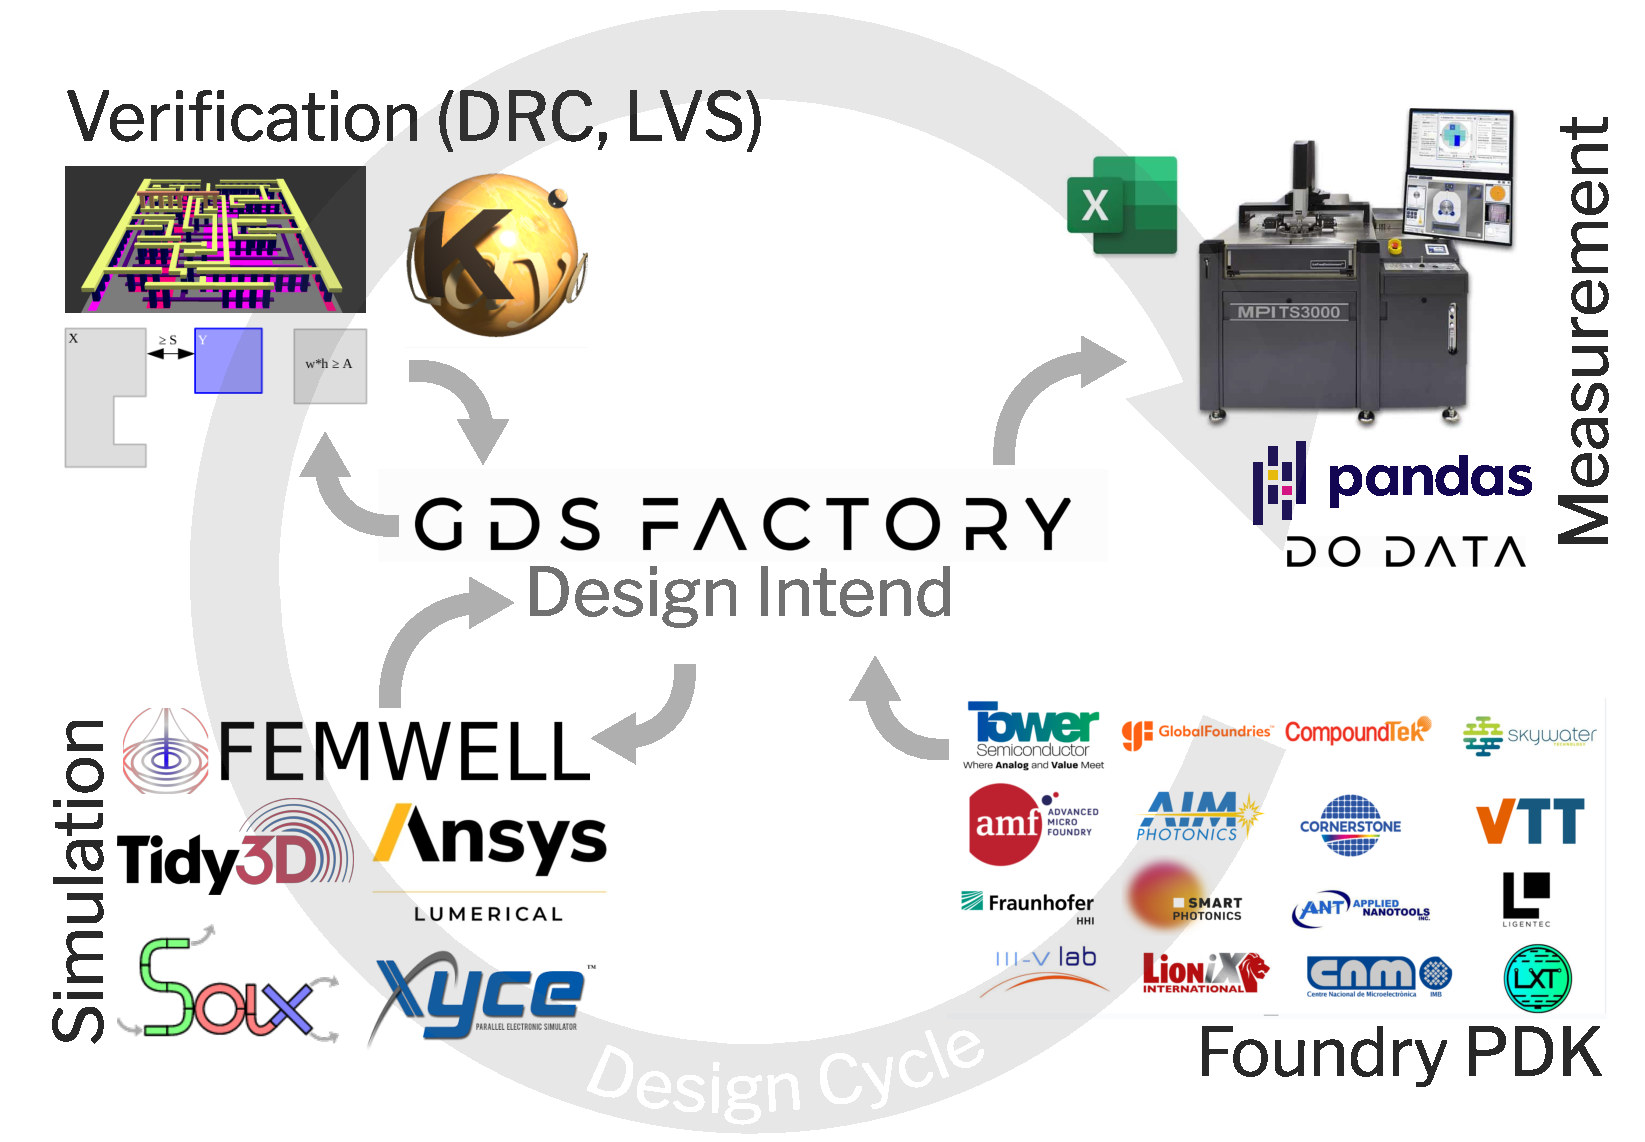
\includegraphics[width=8cm]{figures/flow/design_cycle.pdf}
\caption{GDSFactory workflow: GDSFactory spans the entire design cycle, with a variety of Foundry PDKs available it is both easy to construct circuits reusing proven devices and to realize conceptually new designs. The generated component layouts can be used in various simulators for exploration, optimization and validation. GDSFactory tightly integrates with KLayout, leveraging its advanced design rule checks (DRC) and layout versus schematic (LVS) capabilities. For characterization of the fabricated devices GDSFactory provides rich metadata compatible to commercial wafer probers, including the position and orientation of fiber-to-waveguide couplers.}
\label{fig:flow}
\end{figure}

\section{Layout Design}

GDSFactory implements cells as Python functions that return a \texttt{Component} object holding polygons, electrical and optical port metadata, and convenience methods for export and plotting. Cells are built on KLayout's C++ geometry engine~\cite{klayout} and defined through a functional style in which the \texttt{@gf.cell} decorator caches results to eliminate redundant regeneration. Port metadata drives automatic routing, with dedicated routing functions connecting individual ports or entire groups of ports. Components compose hierarchically and can also be assembled declaratively from YAML netlists, enabling schema-driven and machine-generated layouts.

\section{Device Simulation}

GDSFactory's gplugins repository~\cite{gplugins} provides unified interfaces to a growing list of simulators by reusing the core layout abstractions (Components, LayerStacks, and Ports). For instance, Components can be meshed via Gmsh~\cite{gmsh} (through the Meshwell wrapper~\cite{meshwell}) for cross-sectional or 3D analysis (Fig.~\ref{fig:mesh}). For the rigorous electromagnetic verification that photonics demands, the library supports full-wave analysis through both Finite-Difference Time-Domain (FDTD) and Finite Element Method (FEM) approaches. FDTD is supported through open-source backends including MEEP~\cite{meep} and Luminescent AI, as well as industry-standard solvers such as Tidy3D~\cite{tidy3d} (cloud-based GPU acceleration) and Lumerical FDTD; a plugin for the open-source fdtdx solver is in development~\cite{fdtdx}. FEM-based and multiphysics solvers include Femwell~\cite{femwell} for waveguide mode analysis and thermal simulation, Palace~\cite{palace} for RF and microwave simulation, and MEOW~\cite{meow} for eigenmode expansion. At the device-physics level, TCAD simulation is supported through DEVSIM~\cite{devsim} for semiconductor device physics and Sentaurus for advanced process modeling. % chktex 13

\begin{figure}[htbp]
\centering
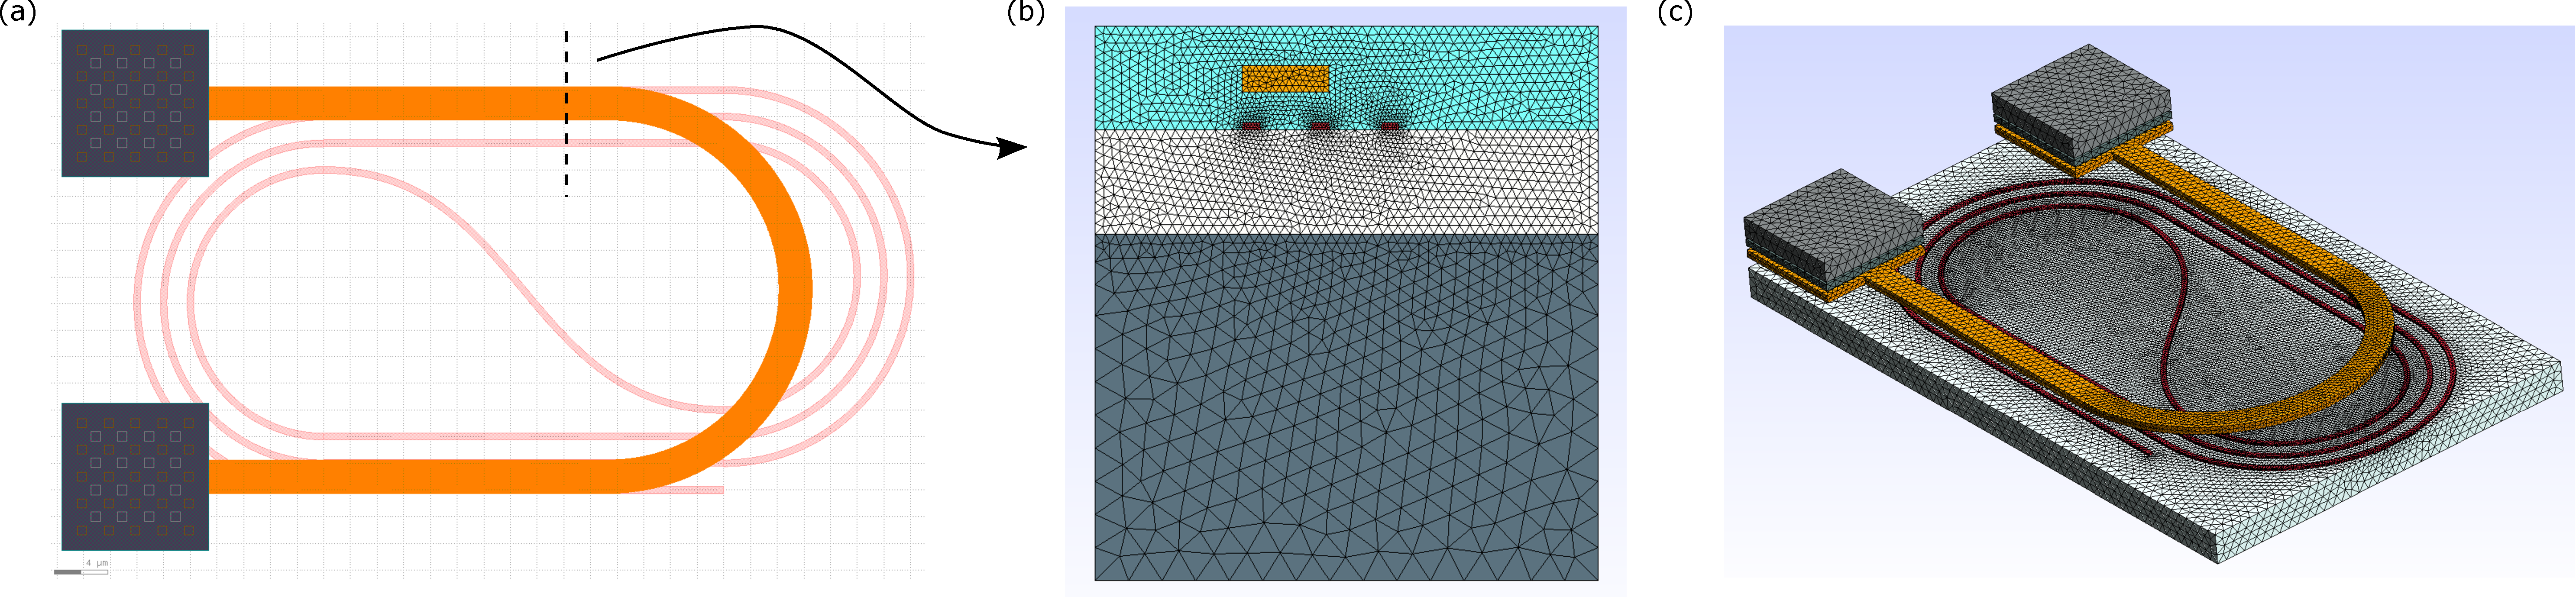
\includegraphics[width=8cm]{figures/gmsh/dessin.pdf}
\caption{GDSFactory meshing: (a) heater layout, (b) cross-sectional mesh, (c) 3D mesh.}
\label{fig:mesh}
\end{figure}

\section{Circuit Simulation}

Circuit-level simulation enables system-scale photonic design. GDSFactory supports this through netlist extraction, which composes device-level models into a full circuit. For example, SAX~\cite{sax} performs differentiable S-parameter simulation on JAX, enabling gradient-based optimization, Monte Carlo analysis for yield estimation, and wavelength-dependent S-parameter interpolation from FDTD results. For mixed photonic-electronic systems, VLSIR~\cite{vlsir} provides SPICE netlist export.

\section{Process Design Kits}

PDKs let GDSFactory drop into existing development flows while matching foundry ground-truth data. Open-source PDKs include GlobalFoundries 180nm, SkyWater 130nm~\cite{skywater}, VTT 3\,\textmu{}m SOI, SiEPIC, Cornerstone, IHP, Luxtelligence, and Quantum-RF-PDK\@. Commercial PDKs available through the GDSFactory+ subscription~\cite{gdsfactoryplus} include AIM Photonics, AMF, CompoundTek, Fraunhofer HHI, Smart Photonics, Tower PH18, OpenLight, III-V Labs, LioniX, Ligentec, Lightium, and QCI\@. For designs not tied to a specific foundry, the generic PDK follows standard layer conventions~\cite{chrostowski2015} for cross-foundry compatibility.

\section{Conclusion}

GDSFactory provides a unified, Python-driven workflow spanning layout, device simulation, and circuit simulation. Tight integration between device solvers and circuit simulators enables rapid iteration from component to system level, and its programmatic, open nature makes it a natural substrate for modern agentic design workflows~\cite{Sharma2025}. The library is freely available at \url{https://github.com/gdsfactory/gdsfactory}.

\begin{thebibliography}{99}

\bibitem{gdsfactory} J. Matres \textit{et al.}, ``GDSFactory,'' GitHub (2024), \url{https://github.com/GDSFactory/GDSFactory}.

\bibitem{bogaerts2018} W. Bogaerts \textit{et al.}, ``Silicon photonics circuit design: methods, tools and challenges,'' Laser Photon. Rev. \textbf{12}, 1700237 (2018).

\bibitem{awesome} J. Matres, ``Awesome Photonics,'' GitHub (2024), \url{https://github.com/joamatab/awesome_photonics}.

\bibitem{klayout} M. K\"offerlein, ``KLayout,'' \url{https://www.klayout.de/}.

\bibitem{gplugins} J. Matres \textit{et al.}, ``gplugins,'' GitHub (2024), \url{https://github.com/gdsfactory/gplugins}.

\bibitem{gmsh} C.~Geuzaine and J.-F. Remacle, ``Gmsh: {A} 3-{D} finite element mesh generator with built-in pre- and post-processing facilities,'' \emph{Int. J. Numerical Meth. Engng}, vol.~79, no.~11, pp. 1309--1331, 2009. [Online]. Available: \url{https://doi.org/10.1002/nme.2579}.

\bibitem{meshwell} S. Bilodeau \textit{et al.}, ``Meshwell,'' GitHub (2026), \url{https://github.com/simbilod/meshwell}.

\bibitem{meep} A. F. Oskooi \textit{et al.}, ``MEEP: A flexible free-software package for electromagnetic simulations by the FDTD method,'' Comput.\ Phys.\ Commun.\ \textbf{181}, 687--702 (2010). % chktex 13

\bibitem{tidy3d} Flexcompute Inc., ``Tidy3D,'' \url{https://www.flexcompute.com/tidy3d/}.

\bibitem{fdtdx} Y. Mahlau \textit{et al.}, ``A flexible framework for large-scale FDTD simulations: open-source inverse design for 3D nanostructures,'' in \textit{Photonic and Phononic Properties of Engineered Nanostructures XV}, vol.~13377, pp. 40--52 (2025), \url{https://github.com/ymahlau/fdtdx}.

\bibitem{femwell} H. Gehring \textit{et al.}, ``Femwell,'' GitHub (2023), \url{https://github.com/HelgeGehring/femwell}.

\bibitem{palace} AWS, ``Palace: 3D Finite Element Solver for Computational Electromagnetics,'' GitHub (2024), \url{https://github.com/awslabs/palace}.

\bibitem{meow} F. Laporte, ``MEOW,'' GitHub (2024), \url{https://github.com/flaport/meow}.

\bibitem{devsim} J.~E. Sanchez, ``{DEVSIM}: {A} {TCAD} {Semiconductor} {Device} {Simulator},'' \emph{Journal of Open Source Software}, vol.~7, no.~70, p. 3898, Feb. 2022. [Online]. Available: \url{https://doi.org/10.21105/joss.03898}

\bibitem{sax} F. Laporte, ``SAX,'' GitHub (2023), \url{https://github.com/flaport/sax}.

\bibitem{vlsir} D. Fritchman \textit{et al.}, ``VLSIR'' GitHub (2024), \url{https://github.com/vlsir/vlsir}.

\bibitem{skywater} SkyWater Technology Foundry and Google, ``SkyWater Open Source PDK,'' GitHub (2023), \url{https://github.com/google/skywater-pdk}.

\bibitem{gdsfactoryplus} GDSFactory, ``GDSFactory+,'' \url{https://gdsfactory.com/}.

\bibitem{chrostowski2015} L. Chrostowski and M. Hochberg, \textit{Silicon Photonics Design} (Cambridge, 2015).

\bibitem{Sharma2025}
A.~Sharma \emph{et al.}, ``AI agents for photonic integrated circuit design automation,'' \emph{APL Machine Learning}, vol.~3, no.~4, Dec.~2025. doi: 10.1063/5.0300741. % chktex 12

\end{thebibliography}

\end{document}
